%%%%%%%%%%%%%%%%%%%%%%%%
%
% $Autor: Wings $
% $Datum: 2019-07-09 09:26:07Z $
% $Pfad: Vorlesungen/WS_19_20/Projekte/KandaNeuralnetwork/latex - Ausarbeitung/Kapitel/Hardware.tex $
% $Version: 4440 $
%
%%%%%%%%%%%%%%%%%%%%%%%%

{\tiny Quelle: \url{https://www.arduino.cc/pro/tutorials/portenta-h7}}


\chapter{Arduino}

\section{Introduction to Arduino}
Arduino is an open-source electronics platform based on flexible, easy-to-use hardware and software. It provide us on board microcontroller and microprocessor kits for making digital and analogue devices. The microcontroller, oftenly called as tiny computer embed on the Arduino board, normally in order to run these microcontroller we need some type of electronics e.g; diodes, resisters, capacitors, and transistors for making the voltage and current balancing. But the arduino team make a user friendly environment for getting rid of these electronics complication to run the hardware on software, just power the board as per the required voltage write the desired programm and upload it in a few seconds, it will bring everything on the board and  make us independent from any worry about the electronics complication. By the technological advancement in semiconductor and electronics  industry, the  control problems are now being solved by using these small size microcontroller instead of mechanical and electrical swithes. All Arduino boards have one thing in common which is a microcontroller, it is basically a really small computer, which help us to make a edge computing application.%\cite{Arduino:2021b}

\section{Arduino Nano 33 BLE Sense}


Arduino Nano 33 BLE Sense is one type of arduino family board, which is come up with bluetooth capability for communication and set of sensors. This compact and reliable Nano board is built around the NINA B306 module for BLE and Bluetooth 5.0 communication; Bluetooth 5.0 is the latest version of the Bluetooth wireless communication standard. Use of microcontrollers has become inevitable in almost every field of engineering.  The Arduino Nano 33 BLE Sense module is based on Nordic nRF52480 processor that contains a powerful Cortex M4F and the board has a rich set of sensors that allow the creation of innovative and highly interactive designs. Its reduced power consumption, compared to other same size boards, together with the Nano form factor opens up a wide range of applications. The following figure ~\ref{Arduino Nano} shows a Arduino Nano 33 BLE Sense, shows how compact it is and small in size.

\begin{figure}[ht]
	\centering
	
\includegraphics[width=0.45\linewidth]{images/Arduino/ArduinoNano33BLESense}
	\caption{Arduino Nano 33 BLE Sense} 
	\label{Arduino Nano}
\end{figure}

Due to the Bluetooth low energy (BLE) and set of sensors which are emded on it, this arduino board makes a perfect match for tiny Machine learning and IOT application. Bluetooth is used for communication between Arduino board and external devices. 

\section{On-Board Sensor Description}

Arduino Nano 33 BLE sense come up with the set of embed sensor on the board. The available embed sensors are commonly use for measuring both the analog and digital values around the sorrounding. Arduino Nano 33 BLE sense is very small (45x18)mm in size, which  makes it very usefull for Internet of things (IOT) and Artificial intelligence (AI) application as a embed device where space is the main constrained issue. It is low power consumption board and operate normally on 3.3 V, we can say that this small size low power consumption board can operate on small batteries even for many months. Due to on-board available sensor, the low power consumption and mini architecture we can use this nano board anywhere. The Arduino Nano 33 BLE Sense is a completely new board on a well-known form factor. For getting detail information about each component of Arduino Nano 33 BLE Sense and data sheets of each sensor the following links give us a detail information %\cite{ArduinoNano33:2021}
. The short description of each sensor are as follow. 

\begin{itemize}
	\item The ADPS-9960 is a digital proximity, ambient light, RGB and gesture sensor. it can measure the proximity distance, light, color and gestures when moving close with the borad.
	\item The LPS22HB is a barometric pressure sensor, it measures the environmental pressure which is usefull for simple weather station monitoring. 
	\item The LSM9DS1 is a 9 axis inertial measurement unit (IMU) use as a Accelerometre, gyroscope, and magnatometre, this 9 axis (IMU) sensor is ideal for wearable devices.
	\item The HTS221 sensor senses the relative humidity, and temperature, to get highly accurate measurements of the environmental conditions.
	\item The MP34DT05 is the digital microphone. it is usefull for capturing, analyzing and detecting the sound in real time.
\end{itemize}

The below figure %\ref{Arduino Nano 33 BLE Sense Architecture}
show the embed sensors on the board, with powerful processor as compared to other arduino boards the nRF52840 from Nordic Semiconductors, a 32-bit ARM® Cortex™-M4 CPU processor running at 64 MHz are as follow.

\begin{figure}[ht]
	\centering
	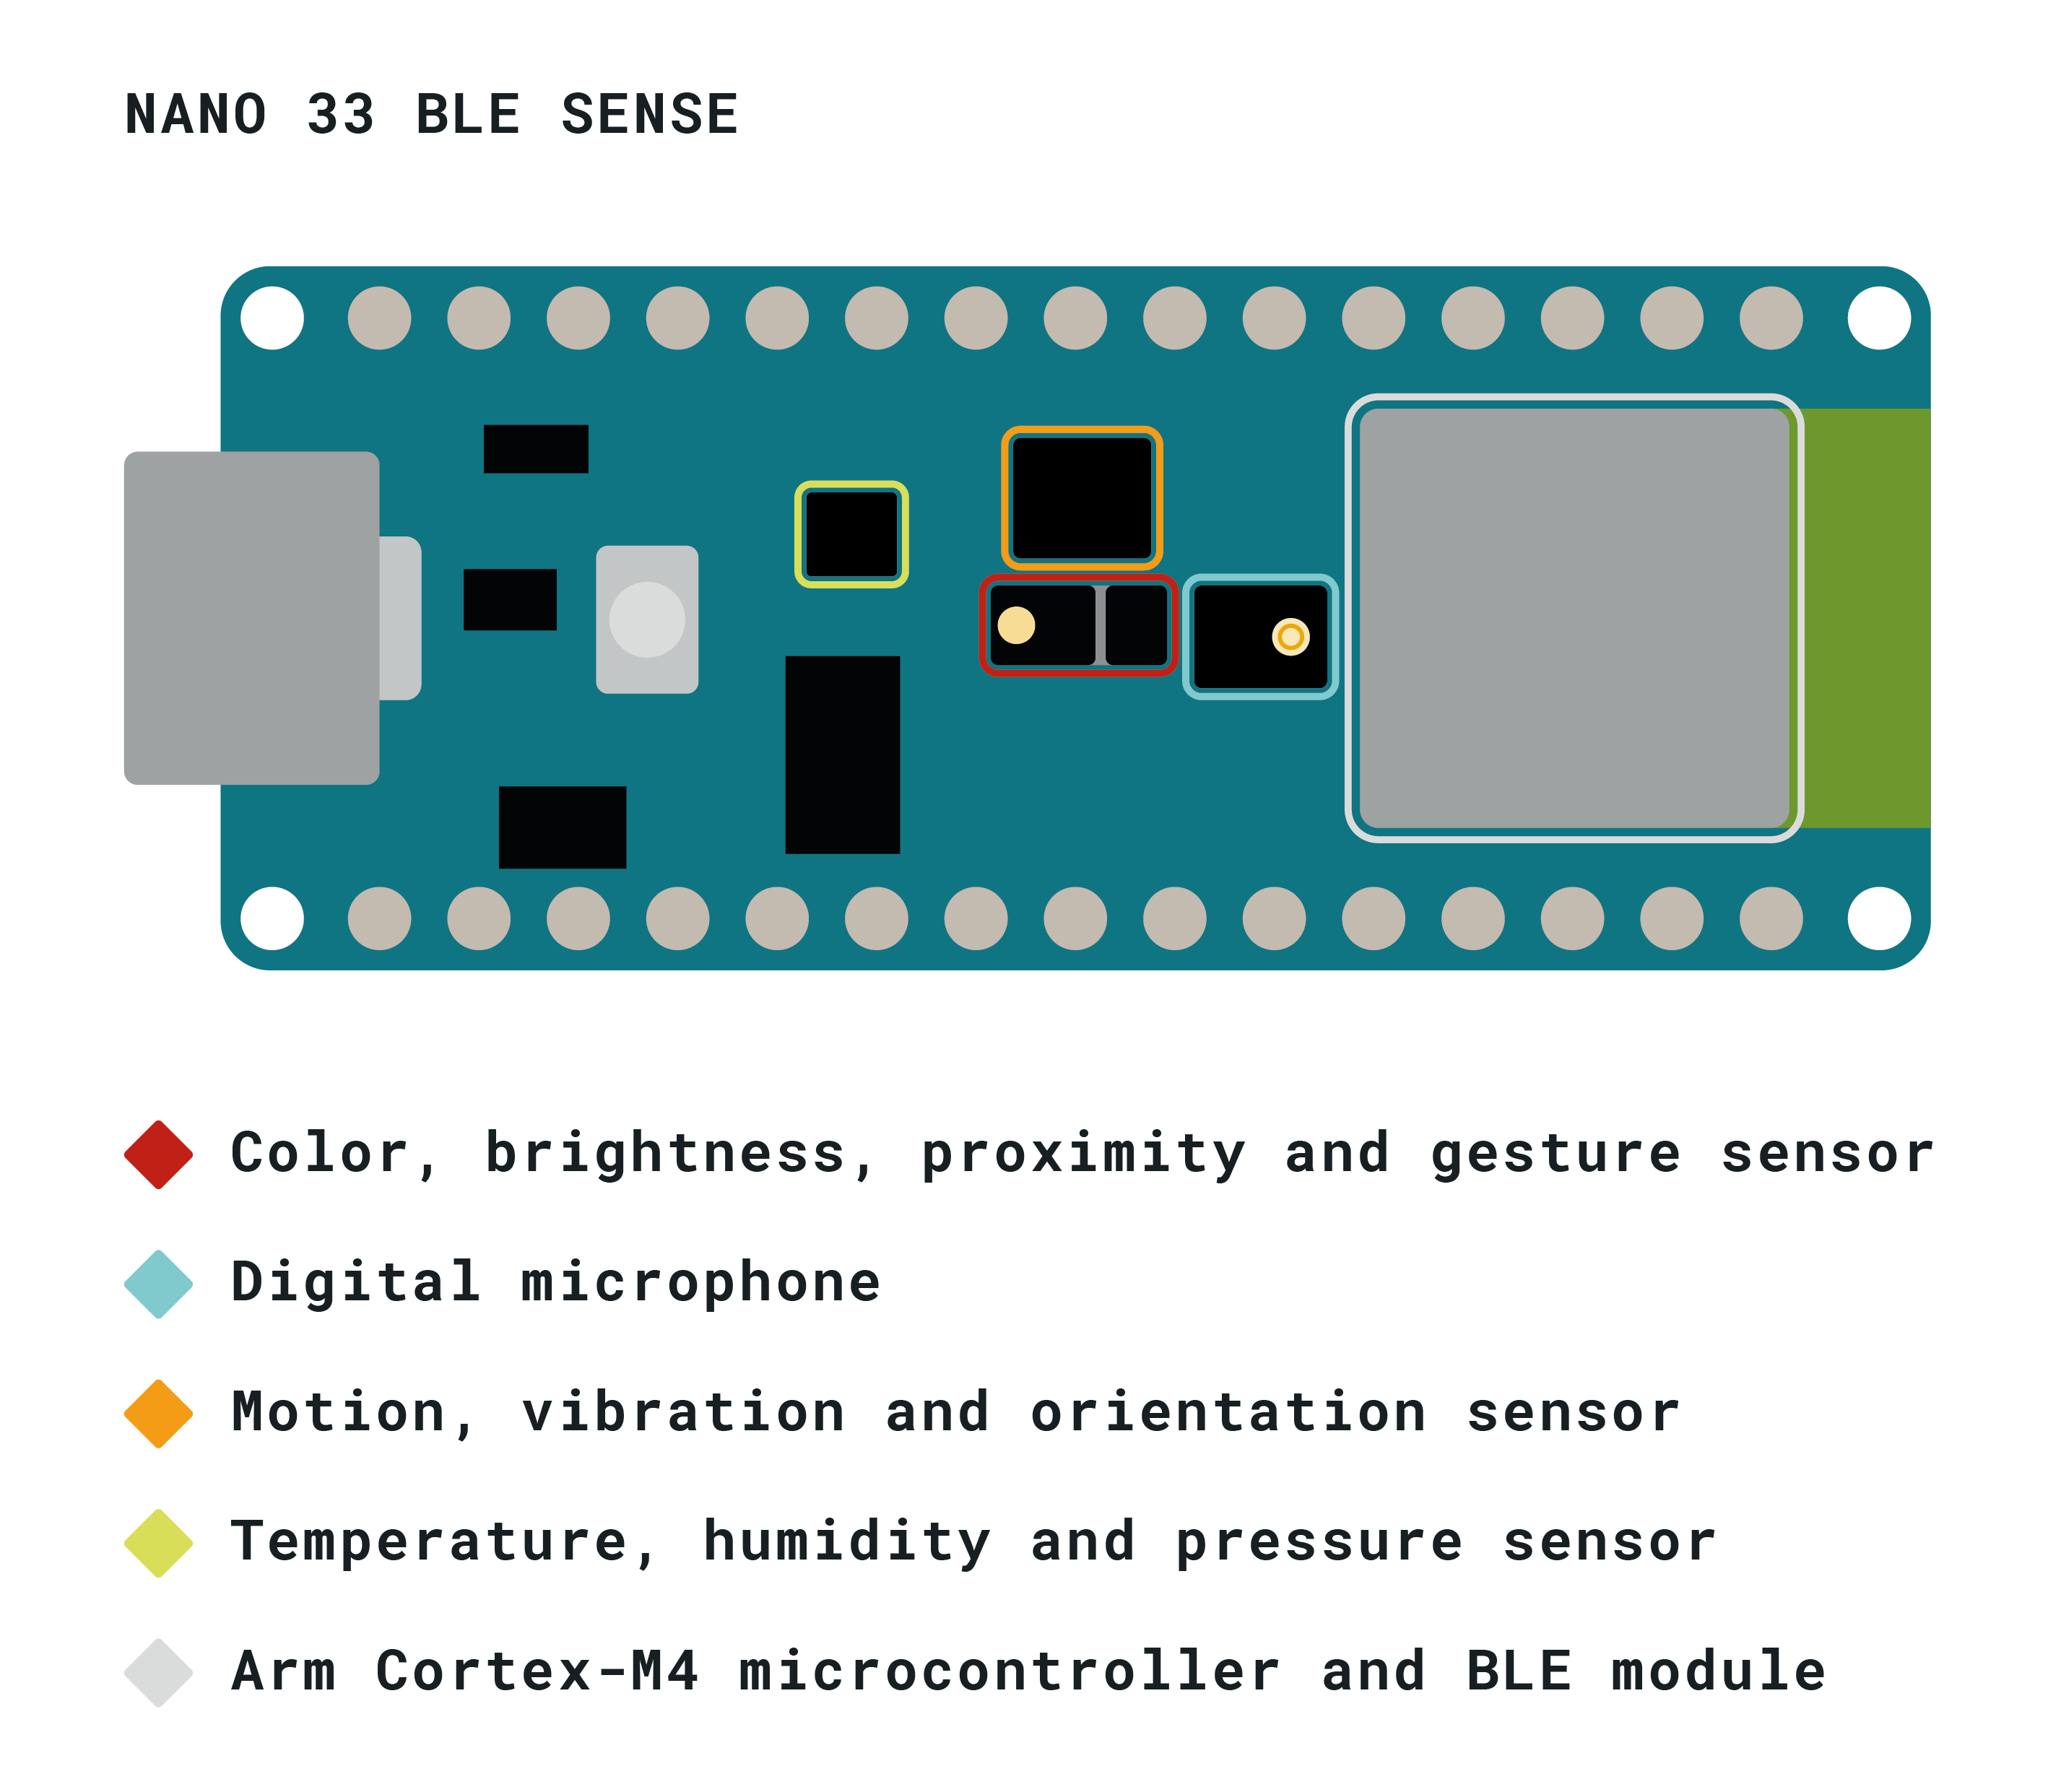
\includegraphics[width=0.5\linewidth]{Images/Nano33BLESense/NANO-33-BLE-Sense_sensor-indentification}
	\caption{Arduino Nano 33 BLE Sense Sensors Placement} 
	\label{Arduino Nano 33 BLE Sense Architecture}
\end{figure}

The Arduino Nano 33 BLE Sense is an evolution of the traditional Arduino Nano, but featuring a lot more powerful processor, the nRF52840 from Nordic Semiconductors, a 32-bit ARM® Cortex™-M4 CPU running at 64 MHz.%\cite{ArduinoNano33:2021} 
This will allow you to make larger programs than with the Arduino Uno (it has 1MB of program memory, 32 times bigger), and with a lot more variables (the RAM is 128 times bigger). The main processor includes other amazing features like Bluetooth® pairing via NFC and ultra low power consumption modes.

\section{General Overview Arduino Board}

Arduino consists of both a physical programmable circuit board (often referred to as a microcontroller) and a piece of software, or Integrated Development Environment (IDE) that runs on our computer, used to write and upload computer code to the physical board. Most of the arduino boards have both analog and digital General purpose input/output (GPIO) pins integrated on the board, depends upon the usage and functionality of the microcontroller embed on arduino board, these multipurpose GPIO makes it more usefull. By the advent of arduino, it make ease and get rid of external programming devices, we dont need to plug in and plug out our microcontrooler for programing the microcontroller. Arduino just need a connection with the computer with the help of USB, and we can upload the programm in a few second. %\cite{Arduino:2021b}

\chapter{TinyML on Arduino Nano 33 BLE Sense}

The integration of machine learning (ML) and artificial intelligence (AI) has become increasingly widespread, with applications spanning across a wide range of industries and fields. These cutting-edge technologies are being employed to streamline processes and enhance accuracy, with a prime example being their use in predictive maintenance within the manufacturing industry.
In the transportation industry, AI is being leveraged to analyze road conditions and pave the way for the development of self-driving cars. In healthcare, the use of ML algorithms for the analysis of medical images, such as X-rays and CT scans, is becoming increasingly common. This is helping to improve the detection and diagnosis of diseases, such as cancer. Additionally, ML can be used to predict cardiac arrest, as demonstrated in a recent study \cite{JMIR:2020}, which validated a developed model for clinical usefulness using data obtained from an electronic medical record hospital in the Emergency Department. The integration of these technologies has the potential to revolutionize the way we approach and solve problems, leading to improved efficiency and effectiveness across various fields..%\cite{Dokic:2020}
 
TinyML pertains to the implementation of machine learning algorithms on small, low-power devices such as microcontrollers and sensors, with an example being the Arduino Nano 33 BLE Sense. Due to their limited computational power and memory, these devices necessitate the use of "Tiny" sized and complexity machine learning models. Some practical applications of TinyML include voice recognition on smart speakers, gesture recognition on wearables, and object detection on cameras.
\subsection{Custom Gesture Recognition Model  for Arduino Nano 33 BLE Sense}

For capturing the gesture data using the on-board 9-axis Inertial measurement unit (IMU), we can make different types of gestures by rotating and changing the position by holding the arduino board in our hand . By doing this, the 9-axis IMU changes the accelerometre, and gyroscope value of the sensor. The limitation for training this model is to hold the board in our hand all the time. But, for the testing purpose it changes the valuse as per the gesture as shown in the figure below %\ref{IMU Sensor Capture Data}
for training the Tiny-Ml model.%\cite{ArduinoNano33:2021}

\begin{figure}[ht]
	\centering
	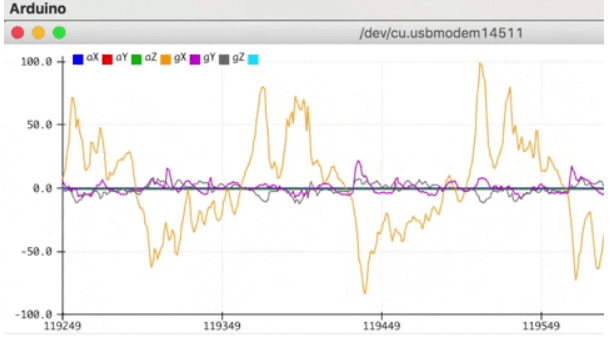
\includegraphics[width=0.5\linewidth]{Images/Nano33BLESense/IMUData}
	\caption{IMU (Inertial Measurement Unit) Gesture Data} 
	\label{IMU Sensor Capture Data}
\end{figure}

The another possibility for detecting gesture is to use the APDS9960 sensor, it can also detect the gesture by moving the hand in front of it. It has also some limitation, it will not detect any gesture above 15 mm distance from the sensor.
\subsection{TensorFlow}

TensorFlow is an open-source deep learning library developed by the Google Brain team in 2015. It is widely used for creating and training machine learning models, catering to both beginners and experts. TensorFlow provides APIs in various programming languages such as Python and C++, making it easy to use for a wide range of applications. While TensorFlow can be used for traditional machine learning tasks, it is particularly powerful for developing complex deep learning applications such as text and image recognition.\\

In 2019, TensorFlow 2.0 was launched, with a focus on ease of use, making it more accessible for developers of all skill levels.\\ 
TensorFlow Lite and TensorFlow Micro, both are versions of TensorFlow that are optimized for deployment on small, low-power devices such as microcontrollers and IoT devices. These versions are suitable for TinyML applications, as they are designed to run efficiently on resource-constrained devices, and can be used to develop machine learning models that are small, fast and power-efficient. \\



- Features
\begin{itemize}
	\item AutoDifferentiation: TensorFlow provides automatic differentiation capabilities, which allow you to easily calculate gradients of a function with respect to its inputs. This is useful for training machine learning models using gradient-based optimization algorithms.
	\item Flexible computation: TensorFlow allows you to perform computations on a variety of devices, including CPUs, GPUs, and TPUs. This makes it easy to scale your computations and take advantage of the available resources.
	\item Large ecosystem: TensorFlow has a large ecosystem of tools and libraries, including TensorFlow Lite and TensorFlow.js, that can be used to perform a wide range of tasks such as training, deploying, and monitoring machine learning models.
	\item Portability: TensorFlow models can be deployed on a wide range of platforms, including mobile devices, web browsers, and servers. This allows you to easily deploy your models in a variety of environments.
	\item Support for multiple languages: TensorFlow provides APIs in multiple languages such as Python, C++, and Java, making it accessible to developers of all skill levels.
	\item Visualization: TensorFlow provides built-in support for visualizing your models and data, which can help you understand and debug your models.
	\item Easy model deployment: TensorFlow provides tools for deploying models to a variety of platforms, including mobile devices and web browsers.
\end{itemize}

Eager execution, Distribute, Losses, Metrics, TF.nn, Optimizers
- Usage and extensions
TensorFlow is both the core platform and a library that one can use for machine learning purposes, Keras an open-source software library written in Python, acts as an interface for the TensorFlow library to make creating machine learning models easier.
%https://www.tensorflow.org/guide/basics
Applications
%https://datasolut.com/einfuehrung-in-tensorflow/
advantages and disadvantages 
Tensorflow can not be used in mobile phones or embedded devices because of the limited memory, 
to avoid this inconvenience, Google also developed TensorFlow Lite a tool that makes it possible to use already trained models on small memory devices 
\subsection{TinyML and Real Time}
The device we are developing requires real-time processing of a person's movement. However, the utilization of TinyML systems presents several challenges in achieving this level of performance. The limited computational power and memory of these devices makes it difficult to run complex machine learning models in real-time, and the storage and processing of large amounts of data can further impede real-time performance. \\
Despite these challenges, it is still feasible to achieve real-time processing using TinyML systems by implementing certain approaches. \\
One approach is to utilize machine learning models that are better suited to the limited resources of TinyML devices.\\
Additionally, techniques such as model quantization, pruning, and compression can be employed to optimize and simplify the model, making it more efficient and better suited to the limitations of the device.\\
Edge computing and on-device processing can also be utilized to reduce the amount of data that needs to be transmitted, stored, and processed, further enhancing real-time performance.

\subsection{TinyMLWorkflow}


%todo GitLab\ToDo\TinyML
% TinyML Seite 222

